\documentclass[linenumber]{jdsart}
\usepackage{setspace}
 
\volume{0}
\issue{0}
\pubyear{2022}
\articletype{research-article}
\doi{0000}

\usepackage{siunitx} % For alignment of numbers
\sisetup{
    group-separator = {,},
    round-mode = places,
    round-precision = 2,
    output-decimal-marker = {.},
    table-number-alignment = center,
    table-figures-integer = 6,
    table-figures-decimal = 2,
    table-figures-uncertainty = 2
}

% image path
\graphicspath{{.}{./images}}

\usepackage{xcolor}
\newcommand{\dt}[1]{\textcolor{purple}{\textbf{DT: (#1)}}}

\let\proglang=\textsf
%% \newcommand{\pkg}[1]{{\fontseries{m}\selectfont #1}}
%% \newcommand\code[2][black]{\textcolor{#1}{\texttt{#2}}}

\usepackage{comment}
\usepackage{subcaption}
\usepackage{booktabs, textgreek}
\usepackage{enumitem}
\usepackage{tikz} % For creating diagrams
\usepackage{hyperref}   % For clickable links and breaking long URLs
\usepackage{url}        % Optional if hyperref is not loaded
\usepackage{fontawesome}
\usetikzlibrary{positioning} % Required for relative positioning (e.g., "of" keyword)
\captionsetup[subfigure]{justification=centering, font=small}

%% float control
\renewcommand\floatpagefraction{0.75}
% \renewcommand\topfraction{.8}
% \renewcommand\bottomfraction{.8}
% \renewcommand\textfraction{.2}
\setcounter{totalnumber}{50}
\setcounter{topnumber}{50}
\setcounter{bottomnumber}{50}


\begin{document}

%\doublespacing 

%\tableofcontents % Optional: Table of Contents
%\listoffigures % List of Figures
%\listoftables % List of Tables


\begin{frontmatter}
  
\title{Detecting Data Anomalies in Open Data: A Case Study with the New
York City 311 Service Request Dataset}
\runtitle{Searching for Data Anomalies}

\author[1]{\inits{D.}\fnms{David}~\snm{Tussey}}
\address[1]{\institution{NYC \textsc{DoITT}}, \cny{USA}}


\hyphenpenalty=950

\begin{abstract}
The open data movement has transformed governance by promoting transparency, 
innovation, and public engagement. Since the 2012 Open Data Law, the City of 
New York (NYC) has been a leader, publishing over 2,400 datasets through its 
Open Data portal. Yet the value of open data depends on its quality—a topic 
often overlooked in the literature.  

This paper presents a case study of anomaly detection within the popular NYC 311 
Service Request (\textsc{SR}) dataset. The analysis reveals that 
uncritical reliance on open datasets 
can yield misleading results. Detection of these anomalies required custom software and iterative 
exploration to uncover patterns not immediately evident.  

Rather than cleaning the data, this study characterizes them, while emphasizing 
that some anomalies—such as a lifecycle of only ten seconds—cannot be judged 
invalid without context. The findings highlight the analytical rigor 
and interpretive judgment necessary to ensure credible insights from open data.
\end{abstract}

\begin{keywords} % no repeating those in title
  \kwd{Data anomalies}
  \kwd{Anomaly detection}
  \kwd{Data quality}
  \kwd{Data validation}
  \kwd{Data curation}
  \kwd{Data cleansing}
  \kwd{Data science}
  \kwd{NYC Open Data}
  \kwd{Smart city}
  \kwd{Transparency}
  \kwd{Government data}
\end{keywords}

\end{frontmatter}

%-------------------------------------------------------------------------------
%	Section: Introduction
%-------------------------------------------------------------------------------

\section{Introduction}
\label{sec:intro}
The open data movement, emerging in the early twenty-first century, rests on 
the premise that freely accessible information can transform governance and 
society by fostering transparency, innovation, and civic engagement. 
A major milestone was the launch of the U.S.\ \textsc{Data.gov} portal in 
2009\,\citep{dataGov}, followed by the European Union’s 
\textsc{Open Data Portal} in 2012\,\citep{dataEU} and the World Bank’s 
\textsc{Open Data} initiative in 2010\,\citep{dataWorldBank}. 
Together, these efforts democratized access to government information and 
encouraged data-driven inquiry across disciplines 
\citep{barns2016mine,wang2016adoption}.  
Yet the effectiveness of open data depends not merely on access but on 
quality, consistency, and usability—issues that remain only partly resolved.

New York City (NYC) has been a municipal leader in this arena since the 
\textsc{Open Data Law} of 2012\,\citep{zuiderwijk2014open}, which established 
the \textsc{NYC Open Data Portal}\,\citep{dataNYC}. 
Hosting more than 2{,}400 datasets across roughly ninety agencies, the portal 
has enhanced governmental transparency and supported extensive research in 
fields such as public health\,\citep{cantor2018facets,shankar2021data}, urban 
development\,\citep{neves2020impacts}, and transportation\,\citep{gerte2019understanding}. 
Datasets on restaurant inspections, traffic collisions, and educational 
enrollment, among others, have informed both policy design and civic 
applications.  In particular, NYC’s 311~Service Request (\textsc{SR}) data have 
been used to optimize resource allocation and improve emergency response, 
demonstrating their operational value.

The size and diversity of these datasets, however, pose persistent challenges 
for data curation—the processes that ensure accuracy, completeness, and 
coherence across time and sources.  High-quality curation underpins effective 
machine-learning models and statistical analyses 
\citep{polyzotis2019data,jain2020overview}, while inadequate practices can 
introduce bias and undermine decision-making 
\citep{geiger2020garbage,rahm2000data}.  
Although open data initiatives emphasize dissemination, the burden of 
verifying and cleaning data often falls to end users 
\citep{cody2017cody,van2018statistical}.  

Research on data curation has advanced understanding of these challenges.  
\citet{witt2009constructing} introduced data-curation profiles for specific 
research contexts; \citet{borgman2012conundrum} examined governance and 
sustainability issues; and \citet{hart2016ten} articulated general principles 
for effective management.  Empirical studies further illustrate the value of 
well-curated data in addressing public-health and crisis-response problems 
\citep{cantor2018facets,shankar2021data}.  Yet large-scale municipal datasets 
remain under-analyzed with respect to systematic quality assessment.

The study addresses this gap through a case analysis of the 
\textsc{NYC 311 SR} dataset.  Rather than attempting to cleanse or correct 
records, this investigation focuses on detecting and characterizing anomalies 
that may compromise analytical validity. This approach 
required custom software, iterative exploration, and 
methodological rigor to uncover patterns not readily visible through routine 
inspection.  Building on these results, we propose a set of practical 
principles for anomaly detection and data assessment tailored to 
government-released open data, with the broader goal of enhancing reliability, 
reproducibility, and interpretability in research and policy contexts.

Section~\ref{sec:service} reviews the history of the NYC~311~system and its 
role as a data source. Section~\ref{sec:data} describes the dataset analyzed. 
Section~\ref{sec:anomalies} details the principal data-quality issues, 
while Section~\ref{sec:principles} outlines recommended 
curation principles.  Section~\ref{sec:conclusion} concludes with key 
findings and implications for future open-data initiatives.

%-------------------------------------------------------------------------------
%	Section: NYC 311 Service Request (SR) Data}
%-------------------------------------------------------------------------------

\section{The New York City 311 Non-Emergency Service} 
\label{sec:service}
The NYC 311 service, a cornerstone of the City’s 
service response framework, functions as a hub for 
non-emergency inquiries, complaints, and requests. Launched in 2003, the system was 
designed to streamline responses to issues ranging from noise complaints 
to street maintenance. Initially limited to phone calls, the service 
expanded to include a mobile application, web portal, text 
messaging, social media, and chat support. Over two decades, 
NYC 311 has evolved into a comprehensive data management platform processing over 3.4 million 
annual requests. 


Beyond its operational function, \textsc{NYC 311} data are
instrumental in shaping City governance and community engagement. 
Open data enhance transparency while empowering civic developers, 
policymakers, and the public\,\citep{minkoff2016nyc,o2017uncharted,kontokosta2021bias}. 
These data have informed crisis management 
(e.g., directing residents to shelters during emergencies, extreme weather events,
 or coordinating COVID-19 responses), improved everyday urban governance 
(e.g., landlord--tenant enforcement, taxi route realignment by the 
Taxi and Limousine Commission (TLC), rodent control, and agency responsiveness), 
Additionally the data has supported a range of academic studies on urban issues, 
including resource allocation\,\citep{zha2014profiling,raj2021swift}, 
social equity in service provision\,\citep{white2018promises,kontokosta2021bias}, 
and environmental challenges \,\citep{dove2022sounds} 
and street flooding\,\citep{agonafir2022understanding}.

%-------------------------------------------------------------------------------
%	Section: 311 SR Dataset Description
%-------------------------------------------------------------------------------

\section{Dataset Description} 
\label{sec:data}
This paper uses a five-year dataset of NYC 311 Service Requests (SRs), 
downloaded from the NYC Open Data Portal on 10 October 2025. 
The dataset main characteristics are:

\begin{itemize}[left=1.5em]
  	\item The raw dataset consists of 16 million records 
  	(9 GB) in CSV format. For efficiency 
	using the R programming language, the file was 
 	converted to the RDS format. Each record 
	has 41 fields, with each row 
	representing a single SR (e.g., complaint or request).
  
	 \item Four date fields are expressed in \texttt{YYYY-MM-DD hh:mm:ss} format. 
  	(Not all agencies track times to the second; some record times only to the minute.)
    		\begin{itemize}
      			\item \texttt{created\_date}
      			\item \texttt{closed\_date}
      			\item \texttt{resolution\_action\_updated\_date} (also \texttt{updated\_date})
      			\item \texttt{due\_date}
    		\end{itemize}
  
  	\item Two borough fields, \texttt{borough} and \texttt{park\_borough}, appear 
  	to duplicate one another.
  
  	\item Seven street-related fields are included, with two pairs of apparent duplicates:
    		\begin{itemize}
      			\item \texttt{incident\_address}
      			\item \texttt{street\_name}
     			 \item \texttt{landmark}
      			\item \texttt{cross\_street\_1}, \texttt{cross\_street\_2}
      			\item \texttt{intersection\_street\_1}, \texttt{intersection\_street\_2}
    		\end{itemize}
  
	  \item Eight incident location fields are included (two of which are geo-coded):
		 \begin{itemize}
    			\item \texttt{incident\_address}
    			\item \texttt{latitude} and \texttt{longitude}
    			\item \texttt{location} (a concatenation of latitude and longitude)
    			\item \texttt{street\_name}
    			\item \texttt{landmark}
    			\item \texttt{block} (NYC tax-related mapping system)
    			\item \texttt{x\_coordinate\_state\_plane} and \texttt{y\_coordinate\_state\_plane} 
         		(State Plane Coordinate System, a NOAA-developed surveying framework)
 	 	\end{itemize}
\end{itemize} 

\begin{table}[tbp]
  \centering
  \caption{Top six agencies by share of Service Requests (2020--2024).}
  \label{tab:big-six-agencies}
  \begin{tabular}{lrr}
    \toprule
    \textbf{Agency} & \textbf{Abbreviation} & \textbf{Share of SRs} \\
    \midrule
    New York Police Department & NYPD & 43\% \\
    Housing Preservation and Development & HPD & 19\% \\
    Department of Sanitation & DSNY & 12\% \\
    Department of Transportation & DOT & 7\% \\
    Department of Environmental Protection & DEP & 5\% \\
    Department of Parks and Recreation & DPR & 4\% \\
    \midrule
    \textbf{Total (Top Six)} & & \textbf{90\%} \\
    \bottomrule
  \end{tabular}
\end{table}

The dataset contains 252 distinct \texttt{complaint\_type} categories.
However, the top twenty complaints 
account for nearly 70\% of all SRs. The complaint distribution is 
highly skewed, with a small number of issues dominating 
overall volume and a long tail of low-frequency complaints. 

Noise-related complaints are especially prominent, represented 
by eight separate categories, including vehicle, residential, commercial, 
and street noise. Taken together, these account for nearly 
one-quarter (23.4\%) of all complaints, making \emph{noise} by 
far the most common issue. Other leading categories 
include illegal parking, heat and hot water complaints, and blocked driveways.

Anomalies in the dataset are typically associated with specific city agencies, 
which facilitates targeted corrective actions. As shown in 
Table~\ref{tab:big-six-agencies}, the six largest agencies account for
nearly ninety percent of all SRs submitted between 2020 and 2024.


%-------------------------------------------------------------------------------
%	Section: Data Cleansing Issues and Anomalies
%-------------------------------------------------------------------------------


\section{Data Cleansing and Anomaly Identification} 
\label{sec:anomalies}
Data cleansing is the process of identifying and correcting errors, 
inconsistencies, anomalies, and inaccuracies to ensure that a dataset is 
sufficiently reliable for analysis\,\citep{maletic2005data,hosseinzadeh2023data}. 
Typical operations include removing duplicates, handling missing values, 
correcting mislabeled entries, and standardizing formats\,
\citep[e.g.,][]{cody2017cody,van2018statistical}. 
For open data, these challenges are amplified by the diversity of sources 
and the lack of coordination across contributing agencies, leading to 
uneven quality and consistency.
When data cleansing is achieved, it enhances trust, supports reliable analysis, and 
facilitates integration into applications such as machine learning. 
This study does not attempt to cleanse the \textsc{NYC 311} dataset but 
instead focuses on the preceding step—systematically detecting and 
characterizing anomalies that may compromise its reliability.

%-------------------------------------------------------------------------------
%	Sub-section: Pre-analysis Data Modifications
%-------------------------------------------------------------------------------

\subsection{Pre-analysis Data Modifications}
\label{subsec:premodifications}
Prior to analysis, the raw dataset undergoes a series of preparatory 
modifications to facilitate efficient processing. These steps 
include both structural adjustments and content standardization:

\begin{itemize}[left=1.5em]
  \item \textbf{Standardization of structure:} 
  Column names are normalized for ease of reference, and the raw 
  \texttt{.csv} file is converted into the more efficient 
  \texttt{.rds} format to improve performance.

  \item \textbf{Date handling:} 
  All date fields are converted to the \texttt{POSIXct} class and aligned 
  to the \textit{America/New\_York} time zone, enabling accurate 
  treatment of Daylight Saving Time (DST) effects 
  (discussed in Section~\ref{par:dst}).

  \item \textbf{Agency harmonization:} 
  Several agencies were renamed during the study period; records were 
  consolidated under their current designations for consistency.

  \item \textbf{Validation of completeness:} 
  Rows are screened for mandatory fields. 
  Missing or absent values—recorded in multiple raw formats—are 
  standardized to \texttt{NA} to facilitate easy in processing.
  Notably, approximately 27\% of the dataset contains missing entries.

  \item \textbf{Field formatting:} 
  Text fields are converted to uppercase for consistent matching, and 
  numeric fields are explicitly cast to the appropriate type.
\end{itemize}


%-------------------------------------------------------------------------------
%	Sub-section: Structural Issues
%-------------------------------------------------------------------------------

\subsection{Structural Issues}
\label{subsec:structural}
Structural issues concern the way data are organized, formatted, or 
encoded---that is, how the dataset is \emph{structured} rather than 
what it \emph{contains}. Structural issues can hinder efficient analysis and often require 
substantial preprocessing before the data can be reliably used. 
In the \textsc{NYC 311} dataset, three notable structural issues were identified:

\begin{itemize}[left=1.5em]
  \item Inconsistent representation of missing-data values
  \item Daylight Saving Time (DST) anomalies
  \item Precision versus accuracy issues in the \texttt{latitude}, \texttt{longitude}, and \texttt{location} fields
\end{itemize}

\paragraph{Inconsistent Representation of Missing Data}
\label{par:missingdata}
The \textsc{NYC 311} dataset exhibits inconsistent conventions for representing 
missing values. Observed forms include nulls, blank spaces, 
``\texttt{NA}'', ``\texttt{N/A}'', and ``\texttt{<NA>}''. 
Such variation complicates programming and analysis, increasing the likelihood 
of errors when filtering or aggregating records. To address this 
issue, all missing values were standardized to \texttt{NA}.

\paragraph{Daylight Saving Time Issues}
\label{par:dst}
The \textsc{NYC 311} dataset records timestamps in New York City local time, 
which observes Daylight Saving Time (DST). 
Twice each year, this practice introduces temporal discontinuities that affect 
the calculation of SR durations, defined as the difference 
between \texttt{closed\_date} and \texttt{created\_date}. 

During the spring transition, local clocks advance from 01:59:59 directly to 
03:00:00, eliminating the entire hour between 02:00:00 and 02:59:59. 
As a result, durations of SRs created before the transition and closed shortly 
afterward are exaggerated by up to one hour. 
While this distortion may appear minor, it is consequential for 
time-sensitive requests such as noise complaints or homelessness-related cases.

During the preprocessing steps several date fields were found to 
violate the DST spring-forward rule, with timestamps recorded during the 
nonexistent hour between 02:00:00 and 02:59:59 
(e.g., \texttt{03/10/2024 02:00:46 AM}, \texttt{03/08/2020 02:10:00 AM}). 
Such values are invalid, as local time advances directly from 01:59:59 to 
03:00:00 on those dates. 
These anomalies were corrected by shifting the affected timestamps forward 
to valid times 
(e.g., \texttt{03/10/2024 03:00:46 AM}, \texttt{03/08/2020 03:10:00 AM}). 
In total, nineteen such corrections were made in the dataset.

The fall DST adjustment introduces a more serious systemic issue by producing 
SRs with \emph{negative} durations, where the 
\texttt{closed\_date} precedes the \texttt{created\_date}. 
Such cases are logically impossible and can distort agency-level performance 
measures, particularly for time-sensitive SRs. 
The following example illustrates the problem:

\begin{itemize}[left=1.5em]
  \item A residential noise complaint SR is created at 01{:}50 on Sunday, March~10,~2024, 
  the date of the DST fall-back transition. 

  \item The \textsc{NYPD} responds promptly, resolving the issue in 
  forty minutes. 
  Without the DST adjustment, the resolution would normally be recorded 
  at 02{:}30.  

  \item However, during this interval the local clock is set back one hour, 
  so the resolution is time-stamped as 01{:}30.  

  \item As a result, the dataset records the SR as closed 
  twenty minutes \emph{before} it was created, yielding a nonsensical
  negative duration of $-20$~minutes.  
\end{itemize}

On average, approximately eighty-six SRs per year exhibit this systemic issue, 
with a mean negative duration of $-42$~minutes.

\paragraph{Precision versus Accuracy in Latitude/Longitude Values}
\label{par:precision}
The \texttt{latitude}, \texttt{longitude}, and the duplicative 
\texttt{location} fields in the raw dataset are recorded with 
fourteen decimal places 
(e.g.,~\texttt{latitude}~$=~40.6409147797767$, 
\texttt{longitude}~$=-73.9736421630642$, 
\texttt{location}~$=(40.640914779776715,\,-73.97364216306418)$). 
Accordingly, 14 decimal points imply positional accuracy at 
the molecular level—an implausible representation. 
This is a case of extreme numerical precision rather than meaningful spatial 
accuracy. For comparison, the official New York City Borough Boundary Water Included
dataset (\textsc{NYBBWI}) published by the Department of City Planning provides 
coordinates to six decimal places, with practical accuracy on the order 
of a few meters. 
(\href{https://s-media.nyc.gov/agencies/dcp/assets/files/pdf/data-tools/bytes/nybbwi_metadata.pdf}{NYC~DCP,~2025}). 
In the present analysis, the original coordinate values were preserved 
without rounding and compared to the official city boundary extents 
(\textsc{NYBBWI}) using a tolerance of approximately \SI{100}{\meter}.


%-------------------------------------------------------------------------------
%	Sub-section: Missing Data by Field
%-------------------------------------------------------------------------------


\subsection{Missing Data by Field}
\label{subsec:blanks}
Understanding the extent and distribution of missing data across fields 
is essential for evaluating the overall usability of the dataset. 
For example, assessing whether SRs were closed before 
their \texttt{due\_date} is largely infeasible, as more than 
\SI{99}{\percent} of entries in this field are blank.  

Additionally, field usage  varies considerably across agencies.
For instance, \texttt{landmark} and \texttt{facility\_type} are 
widely used across agencies, underscoring their importance in 
classifying service requests (SRs). 
By contrast, fields such as \texttt{taxi\_pick\_up\_location} are used 
exclusively by the Taxi and Limousine Commission (\textsc{TLC}). 

Table~\ref{tab:missing-data} summarizes the extent of missingness across 
the dataset, grouping fields by the proportion of blank entries and 
providing representative examples within each category.

\begin{table}[tbp]
  \centering
  \caption{Categories of missing data by field in the NYC~311 SR dataset.}
  \label{tab:missing-data}
  \small
  \begin{tabular}{lll}
    \toprule
    \textbf{Category} & \textbf{Percentage blank} & \textbf{Representative fields} \\
    \midrule
    Mostly empty      & 94--99.9\%   & \texttt{taxi\_company\_borough}, \texttt{due\_date}, \\
                      &              & \texttt{road\_ramp}, \texttt{bridge\_highway\_name} \\
    Partially empty   & 56--93\%      & \texttt{location\_type}, \texttt{address\_type}, \\
                      &              & \texttt{landmark}, \texttt{cross\_street\_1/2} \\
    Few or none empty & 0--55 \%       & \texttt{created\_date}, \texttt{complaint\_type}, \\
                      &              & \texttt{agency} \\
    \bottomrule
  \end{tabular}
\end{table}

Figure~\ref{fig:blank_fields} depicts the proportion of missing values 
across fields, illustrating their distribution into Mostly Empty, 
Partially Empty, and Few/None Empty categories.

\begin{figure}[tbp]
	\centering
  	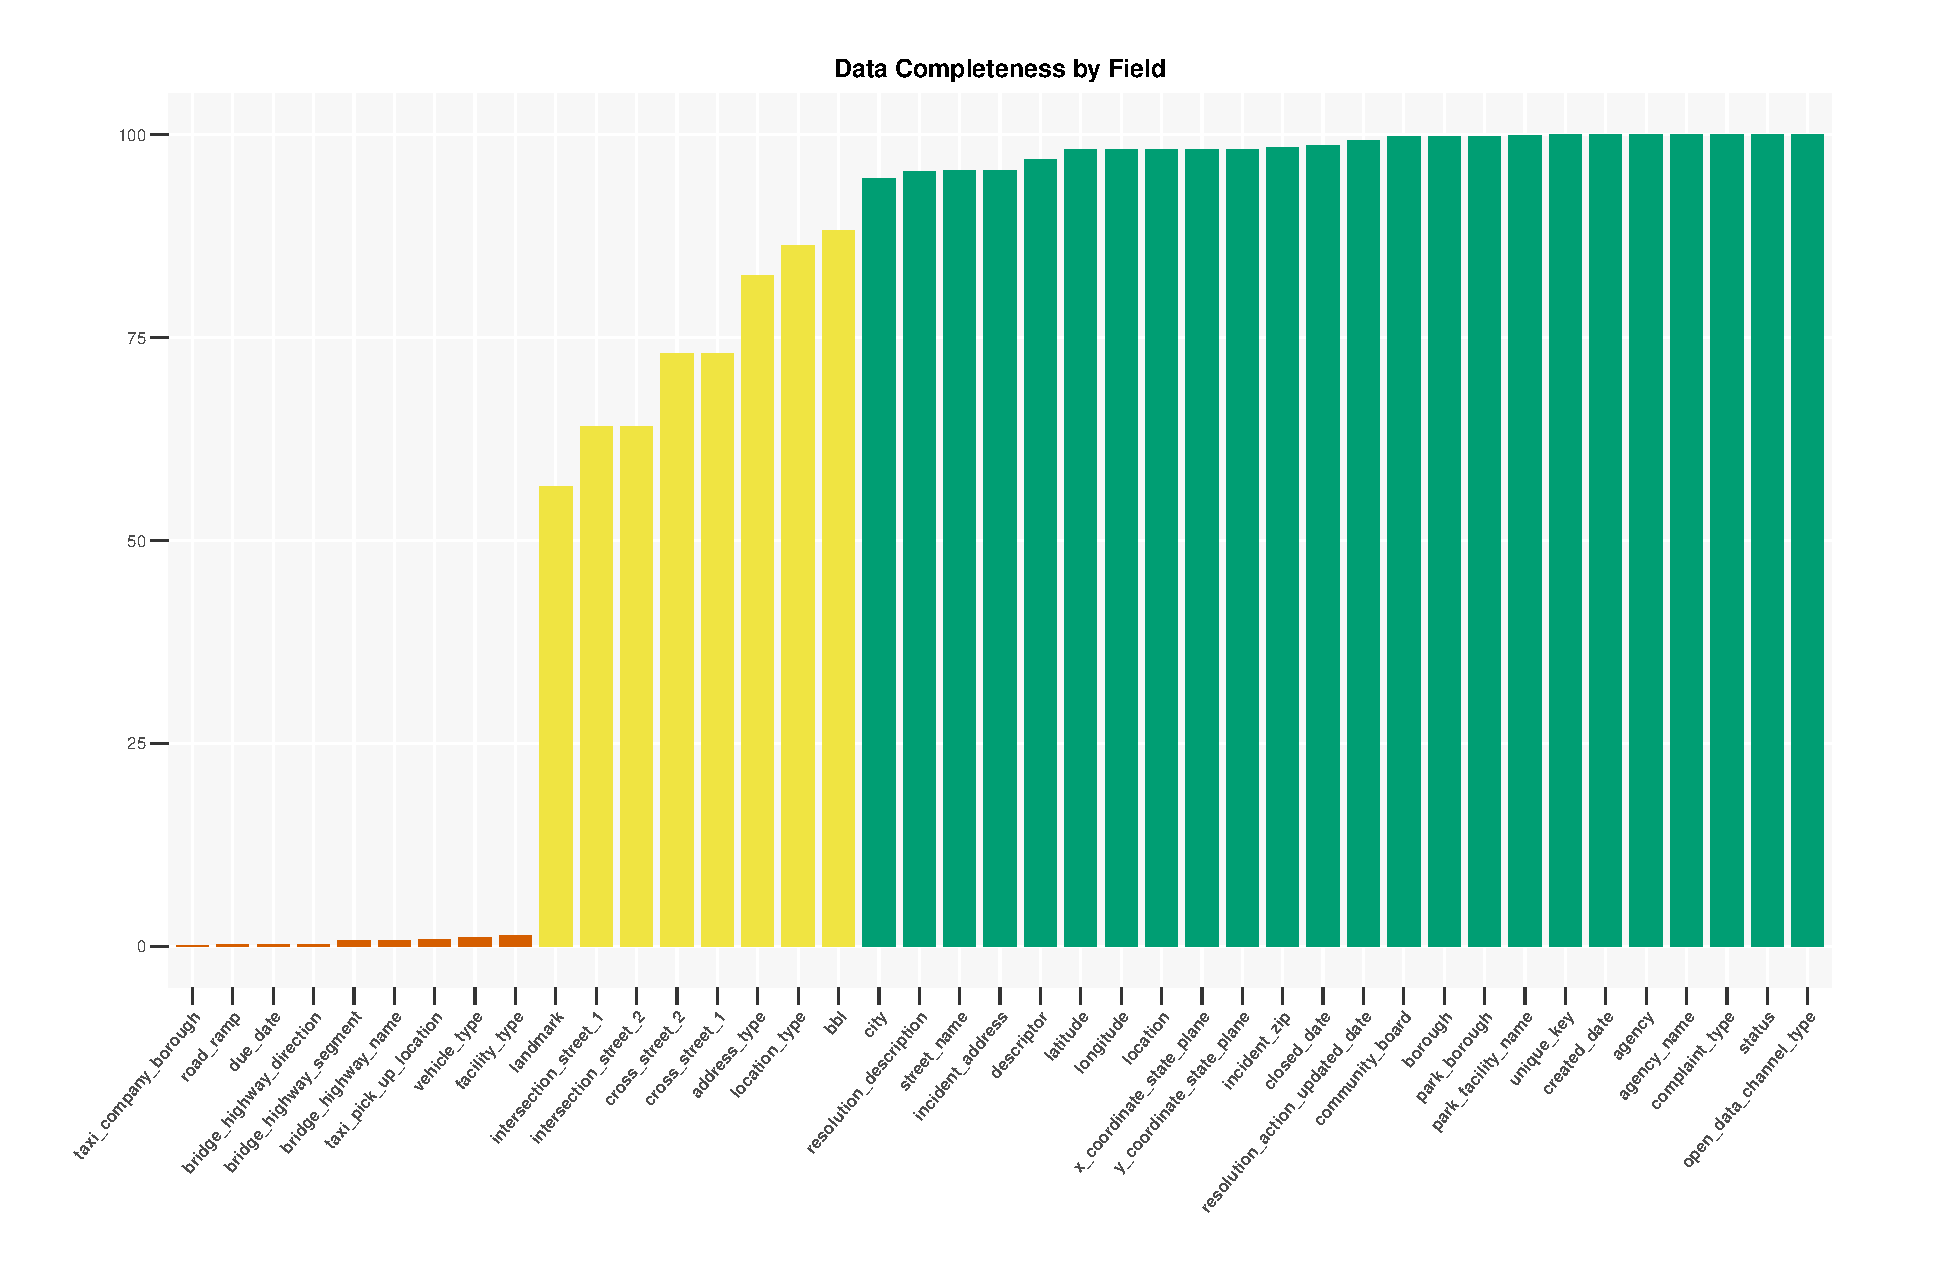
\includegraphics[width=0.7\textwidth, height=0.33\textheight, keepaspectratio]{data_completeness_by_field_bar_chart.pdf}
	\caption{Number and percentage of missing entries for the
          311 SR data (2020--2024)}
	\label{fig:blank_fields}
\end{figure}


%-------------------------------------------------------------------------------
%	Sub-section: Validating Data for Compliance with Allowable Values
%-------------------------------------------------------------------------------

\subsection{Validating Data for Compliance with Allowable Values}
\label{subsec:domain}

\paragraph{Validating Data Type}
\label{par:validatingdatatype}
The 311~\textsc{SR} Data Dictionary, last updated in~2023, 
provides only limited information regarding the data type or class of each 
field, although most can be reasonably inferred. 
The NYC~Open~Data Portal supplements this documentation by indicating field 
types with icons: 
\textbf{T}{\scriptsize\textbf{T}} for text, 
\emph{\textbf{\#}} for numeric, 
\faCalendar\ for date or time fields, 
and \faMapMarker\ for geospatial data.

In most cases, these indicators are sufficient for validation. 
However, the \texttt{incident\_zip} field is labeled with the text emblem 
(\textbf{T}{\scriptsize\textbf{T}}), even though ZIP codes are better 
regarded as fixed--length, numeric but non-computational identifiers. 

All other fields validated properly against their expected data types, as 
determined from the 311~\textsc{SR} Data Dictionary and 
the NYC~Open~Data Portal descriptions. 
More generally, analytic work requires that fields contain values that are 
valid, bounded, and compliant with a domain of known or legal values. 
For some fields, the 311~\textsc{SR} Data Dictionary provides explicit 
definitions; for others, valid domains must be inferred from public usage, 
additional research, or comparison with external datasets. All 
fields examined here were compliant with their known value domains.

The following fields were validated against known domains and found to be 
compliant. They can be grouped into three categories:


\begin{itemize}[left=1.5em]
  \item \textbf{Organizational fields:} 
        \texttt{agency}, \texttt{status}, 
        \texttt{open\_data\_channel\_type}, and \texttt{vehicle\_type}.
  \item \textbf{Geographic fields:} 
        \texttt{borough}, \texttt{park\_borough}, 
        \texttt{city\_council\_district}, and \texttt{taxi\_company\_borough}.
  \item \textbf{Address-related fields:} 
        \texttt{address\_type}.
\end{itemize}

\paragraph{Zip Codes}
\label{par:zipcodesissues}
Validation of the \texttt{incident\_zip} field is relatively straightforward, 
as the U.S.~Postal Service (\textsc{USPS}) maintains a definitive database 
of 42{,}735 valid ZIP~codes. 
Within the NYC~311 dataset, however, 3{,}274 entries were found to be invalid, 
including clearly erroneous values such as \texttt{10000}, \texttt{00083}, 
and \texttt{11111}. 
Although these represent only \SI{0.02}{\percent} of all records, 
the presence of invalid ZIP~codes is notable because this field is among the 
easiest to validate against an authoritative reference. 
Such anomalies highlight the importance of incorporating automated domain 
checks, particularly for fields governed by well-defined external standards.

\paragraph{Community Boards:}
\label{sec:communityboardissues}
The \texttt{community\_board} field captures one of 
New~York~City’s subdivisions of local governance. 
Validation should be straightforward, as there is a publicly 
available list of community boards. 
Nonetheless, this analysis identified 56{,}914 invalid entries, 
representing values outside the accepted set. 
Such anomalies underscore the risks that arise when categorical fields 
linked to well-defined administrative structures are not systematically 
validated.


%-------------------------------------------------------------------------------
%	Sub-section: Date Field Issues
%-------------------------------------------------------------------------------


\subsection{Date Field Issues:}
\label{subsec:datefieldissues}
In addition to the DST-related structural anomalies discussed in 
Section~\ref{par:dst}, the dataset exhibits a range of problems 
specific to its date fields. 
Dates should follow a logical temporal sequence—for example, the 
\texttt{created\_date} should precede the \texttt{closed\_date}. 
The NYC~311 dataset includes four such fields: 
\texttt{created\_date}, \texttt{due\_date}, \texttt{updated\_date}, 
and \texttt{closed\_date}, which are presumably populated in that order. 
In practice, however, numerous records violate these expected relationships, 
introducing inconsistencies that complicate both analysis and interpretation.

\subsubsection{Created Date }
\label{subsubsec:createddate}
All \texttt{created\_date} values were checked to ensure that none were set 
in the future or before the inception of the 311~system (circa~2003); all 
records were compliant. 
However, the analysis identified a notable clustering of timestamps at 
exactly midnight (14{,}409~cases) and exactly noon (31{,}872~cases), 
an anomaly that will be examined further in 
Section~\ref{subsubsec:midnightnoonissues}.

\subsubsection{Due Date Anomalies:}
\label{subsubsec:duedate}
The \texttt{due\_date} field is rarely populated, appearing almost 
exclusively in Department of Sanitation (\textsc{DSNY}) records and 
only about \SI{0.3}{\percent} of the time. 
All values passed validation checks (no dates in the past or implausible 
future), and no unusual temporal patterns were observed.

Sixteen cases were identified in which the \texttt{due\_date} precedes the 
\texttt{created\_date}---a nonsensical condition. These premature 
dates ranged from just over one year early to more than 
two years early. 
Any analysis incorporating such values would produce distorted results, 
particularly when evaluating timeliness against stated deadlines. 
Given that this field is rarely used (the third least populated in the 
dataset, at only \SI{0.3}{\percent} overall), such anomalies are unlikely 
to have a major impact on aggregate analyses but should nonetheless be 
excluded when encountered.

\subsubsection{Closed Date }
\label{subsubsec:closeddate}
There are substantial issues associated with the 
\texttt{closed\_date} field. 
All values were checked to ensure that none were set in the future or 
before the inception of the 311~system (circa~2003); all records were 
compliant in this respect. 
However, the analysis identified a notable clustering of timestamps at 
exactly midnight (14{,}409~cases) and exactly noon (31{,}872~cases), 
an anomaly that will be examined further 
in Section~\ref{subsubsec:midnightnoonissues}


\subsubsection{Resolution Action Updated Date Anomalies:}
\label{subsubsec:resolutionupdatedate}
The \texttt{resolution\_action\_updated\_date} field records the 
datetime when an \textsc{SR} is modified or updated. 
No values were found to lie in the implausible past or future. 
However, 376{,}155~entries (\SI{2.35}{\percent}) occur 
\emph{before} the corresponding \texttt{created\_date}. 
Nearly \SI{80}{\percent} of these early updates fall within a 
single day of creation—many within minutes or even seconds—suggesting 
a potential system-level issue in which the field is populated 
prematurely. 

A more substantive irregularity arises in post-closure updates. 
While such updates are relatively common 
(\SI{54}{\percent} of all updates occur after the 
\texttt{closed\_date}), 27{,}810~records were found in which the update 
occurred more than 30~days—and in some cases up to 1{,}593~days 
(\textgreater4~years)—after closure. 
A Pareto analysis by agency indicates that over \SI{80}{\percent} of these 
late updates are concentrated within the 
Taxi~\&~Limousine Commission (\textsc{TLC}), 
Department of Parks~\&~Recreation (\textsc{DPR}), 
and Department of Health~\&~Mental~Hygiene (\textsc{DOHMH}). 
This clustering raises the question of whether such delays represent 
routine administrative practices or potential data quality issues.

Finally, 91~records exhibit \emph{extremely} late post-closure updates,
linked to invalid \texttt{closed\_date} values set to 1899 or~1900.
These cases likely stem from the well-documented SQL
default-date error in handling blank fields.
Such artifacts should be identified and excluded to prevent
severe distortions in any downstream analysis
(as illustrated in Figure~\ref{fig:extreme-positive-boxplot}).


\begin{figure}[tbp]
  \centering
  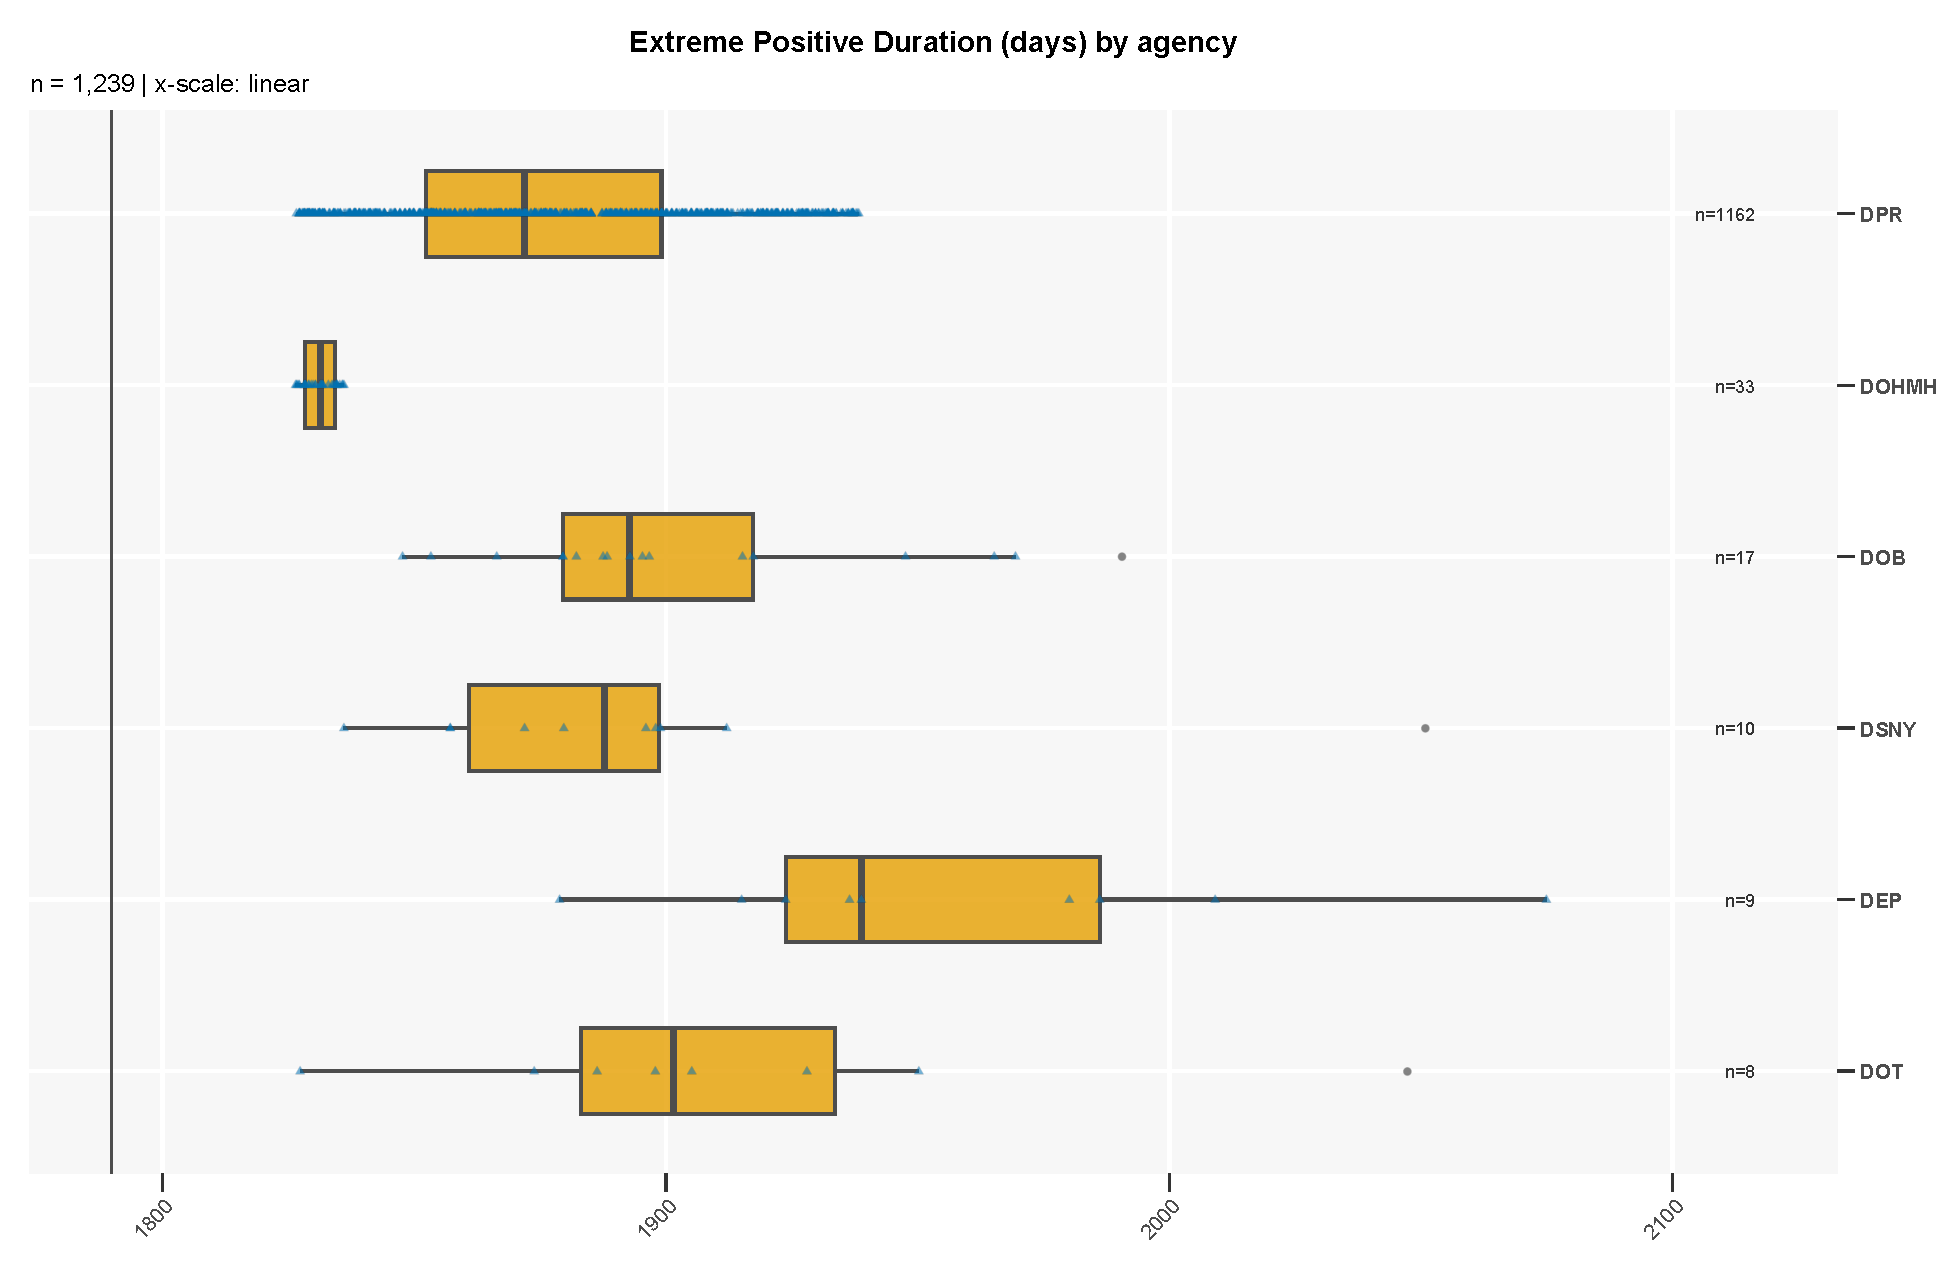
\includegraphics[width=\textwidth]{boxplot_extreme_positive_days_by_agency.pdf}
  \caption{Boxplot of extremely large positive durations (in days) by agency.}
  \label{fig:extreme-positive-boxplot}
\end{figure}


\subsubsection{Daylight Saving Time (DST) Anomalies:}
\label{subsubsec:dst}
The American practice of observing Daylight Saving Time (DST) 
introduces systemic challenges in measuring 
\textsc{SR} durations. 
As noted in Section~\ref{par:dst}, the fall--back adjustment 
imparts nonsensical \emph{negative} durations in roughly 
86~\textsc{SR}s per year, when \texttt{closed\_date} 
precedes \texttt{created\_date}.  

The spring--forward adjustment, by contrast, inflates 
\textsc{SR} durations. At 02{:}00~local time, clocks are 
advanced directly to 03{:}00, creating an artificial one-hour gap. 
Any \textsc{SR}s active (e.g., with status 
\texttt{OPEN}, \texttt{PENDING}, \texttt{IN~PROGRESS}, or 
\texttt{STARTED}) before the transition and subsequently closed 
appear one hour longer in duration than in reality. 
This analysis found that approximately 55{,}000~\textsc{SR}s 
annually are affected by this error.  

Although discrepancies of $+1$~hour or $-42$~minutes may seem minor, 
they can meaningfully distort performance assessments for 
time-sensitive issues. Examples include 
\texttt{Noise--Residential}, \texttt{Animal--Abuse}, 
\texttt{Homeless~Person~Assistance}, and 
\texttt{Drug~Activity}, where response time is a critical measure 
of agency effectiveness. 
These systemic anomalies underscore the need to explicitly account 
for DST when analyzing \textsc{SR} durations.

\subsubsection{Midnight and Noon: Creation and Closure Issues}
\label{subsubsec:midnightnoonissues}
Overall, 311~\textsc{SR} activity follows a typical
daily cycle, with most requests created between 08{:}00 and 23{:}00
(see Figure~\ref{fig:created-hour-dist}).
Closer inspection of the \texttt{created\_date} and
\texttt{closed\_date} fields, however, reveals a distinct temporal
artifact in which unusually large numbers of records occur precisely at
midnight (00{:}00{:}00) and noon (12{:}00{:}00). Such perfect alignment is highly
unlikely to result from human activity and instead suggests that
automated system routines are creating or closing batches of
\textsc{SR}s at these times. While this behavior may not represent an
error per~se, it reflects a systemic process artifact that can distort
analyses of hourly workload, duration distributions, and agency
performance metrics.

As shown in Figures~\ref{fig:exacthours}\subref*{fig:created_top_hour}~and~%
\subref*{fig:closed_top_hour}, both the creation and closure events display
a pronounced concentration at exactly midnight and noon, far exceeding the
expected random frequency and well above \( +3\sigma. \) 

\begin{figure}[tbp]
  \centering
  \begin{subfigure}[b]{0.48\textwidth}
    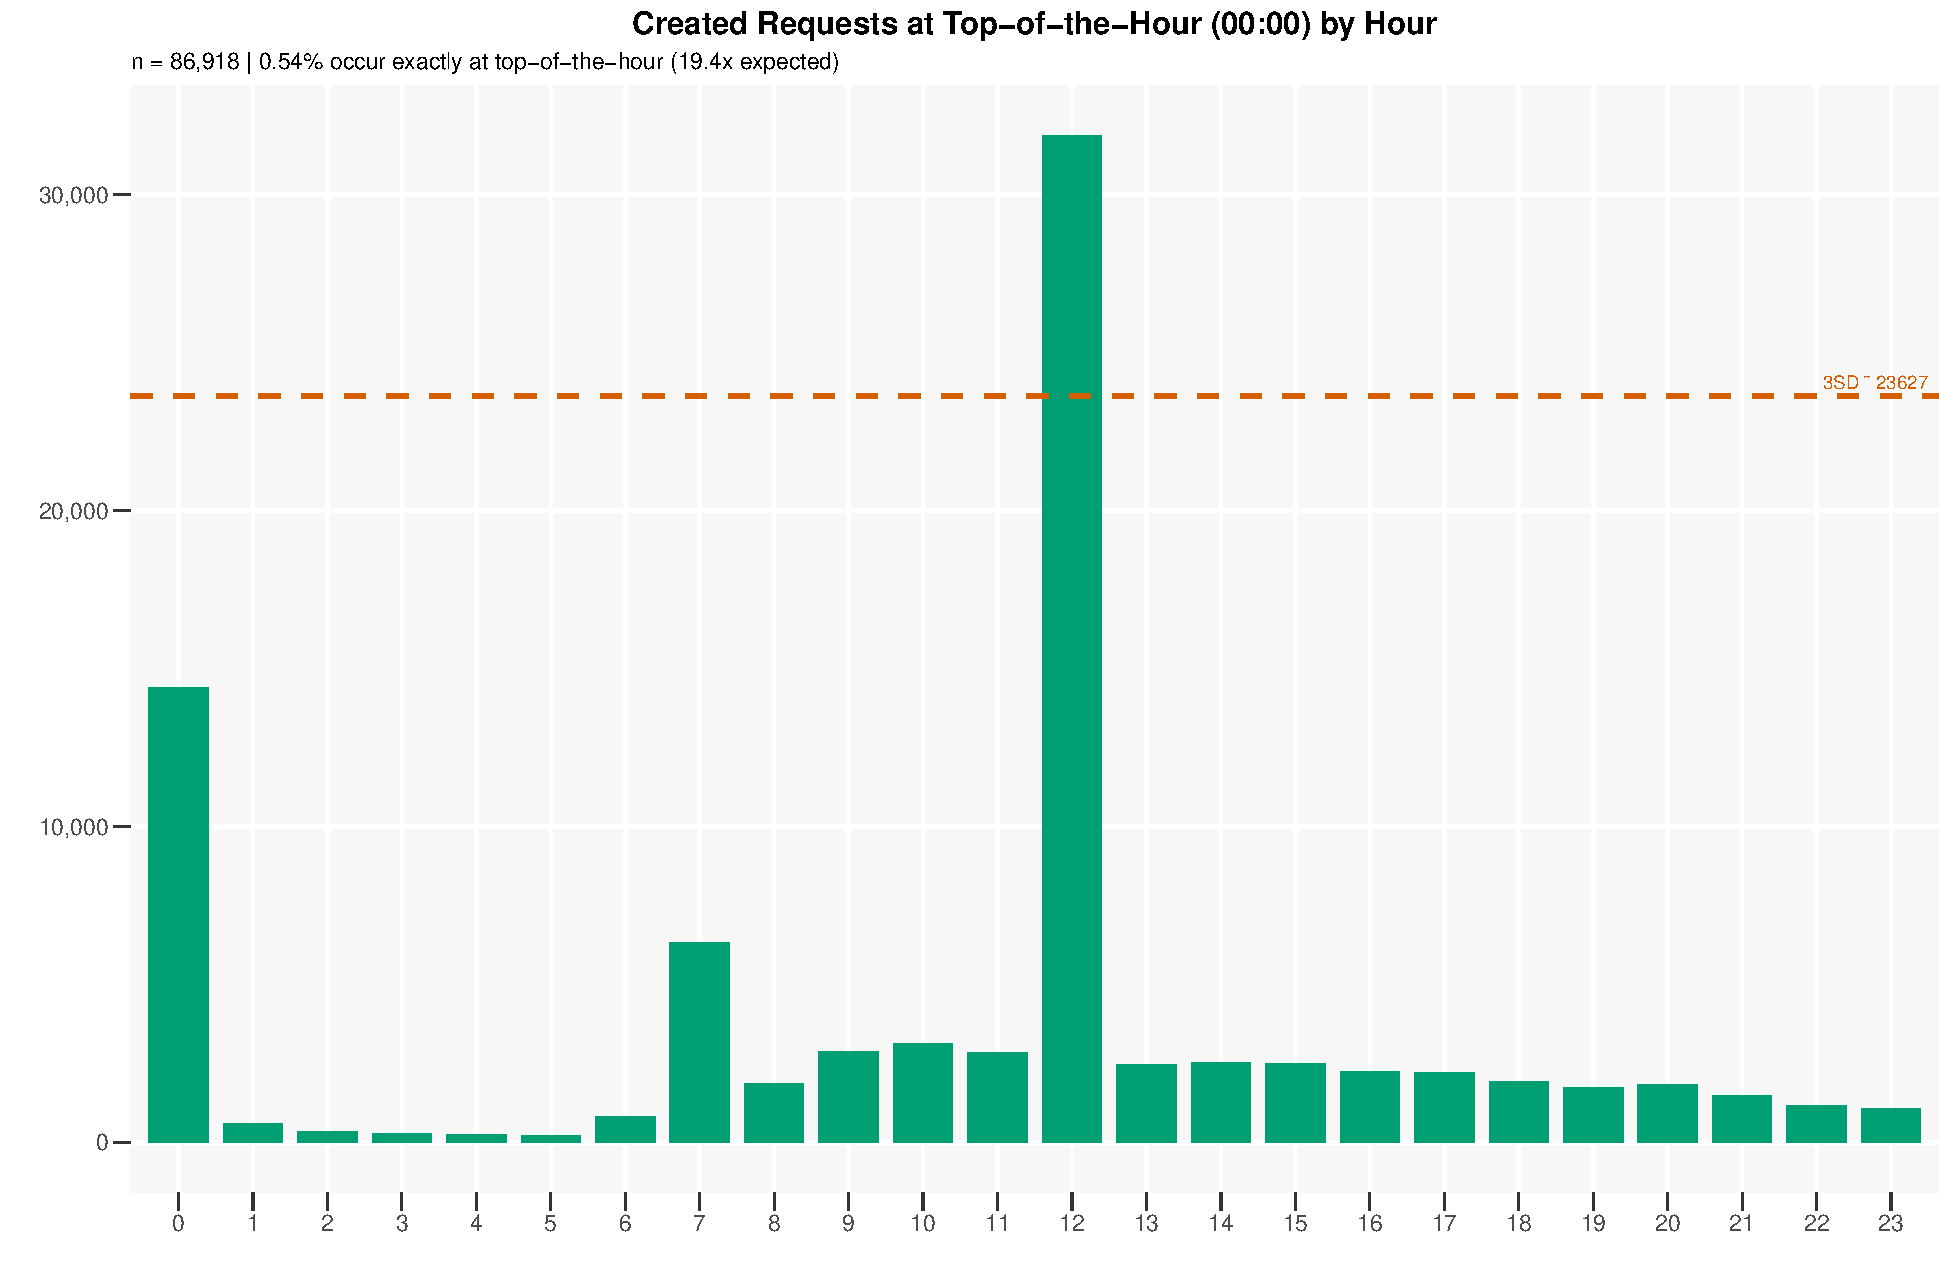
\includegraphics[width=\textwidth]{created_top_of_hour_distribution.pdf}
    \caption{SRs created at the top of the hour (hh{:}00{:}00).}
    \label{fig:created_top_hour}
  \end{subfigure}
  \hfill
  \begin{subfigure}[b]{0.48\textwidth}
    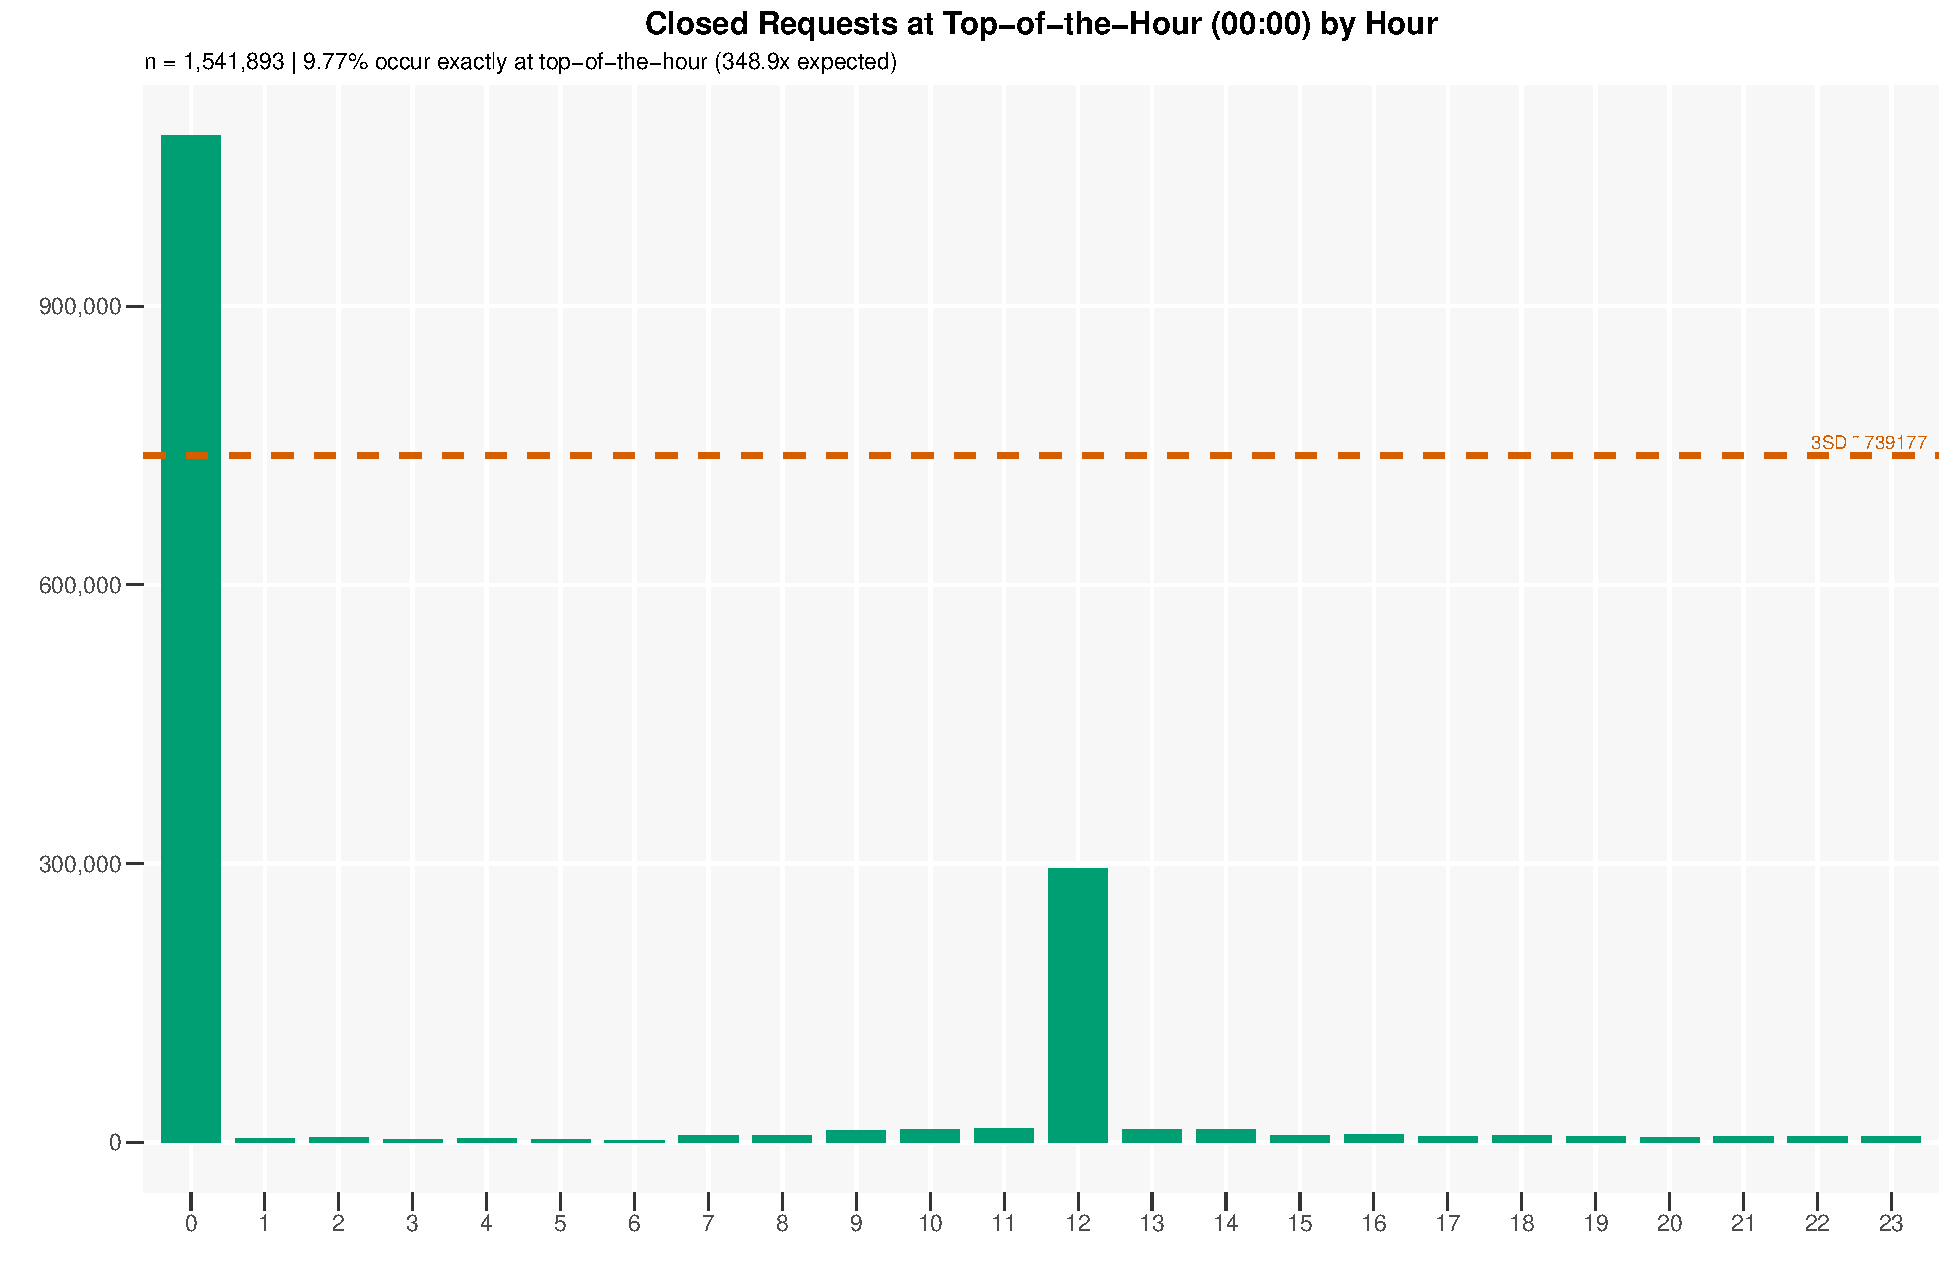
\includegraphics[width=\textwidth]{closed_top_of_hour_distribution.pdf}
    \caption{SRs closed at the top of the hour (hh{:}00{:}00).}
    \label{fig:closed_top_hour}
  \end{subfigure}
  \caption{311~(\textsc{SR}s) created and closed exactly
  at the top of the hour (hh{:}00{:}00).}
  \label{fig:exacthours}
\end{figure}

 \subsection{Duration Issues}
\label{subsec:duration}
The life span of an \textsc{SR}—its 
\textit{duration}—is widely used as a performance metric for 
New~York~City (\textsc{NYC}) agencies. 
Duration is frequently employed to assess equity in service provision 
across neighborhoods, communities, and boroughs, and is often cited in 
City reports as a proxy for agency responsiveness. 
For these reasons, \textsc{SR} duration warrants careful analysis.  

In principle, duration is the elapsed time between the 
\texttt{created\_date} and \texttt{closed\_date} fields. 
Given the prevalence of automated systems, one might expect these fields 
to be populated directly by application software in response to user actions, 
thereby minimizing human error and enforcing basic temporal logic. 
However, this is not consistently the case. 
The dataset contains several anomalies in the 
\texttt{created\_date} and \texttt{closed\_date} fields that would 
ordinarily be prevented by well-designed automation. 
These anomalies raise concerns about the reliability of duration as a 
performance indicator and underscore the need for closer scrutiny.

\subsubsection{Negative Durations:}
\label{subsubsec:negativedurations}
A total of 45{,}296~service requests (\textsc{SR}s) exhibit a 
\texttt{closed\_date} that precedes the \texttt{created\_date}, 
producing nonsensical negative durations. 
More than \SI{98}{\percent} of these anomalies originate from a single 
agency—the Department of Transportation (\textsc{DOT}). 
Across all affected \textsc{SR}s, negative durations average $-119$~days, 
a nontrivial distortion.  

\begin{figure}[tbp]
    \centering
    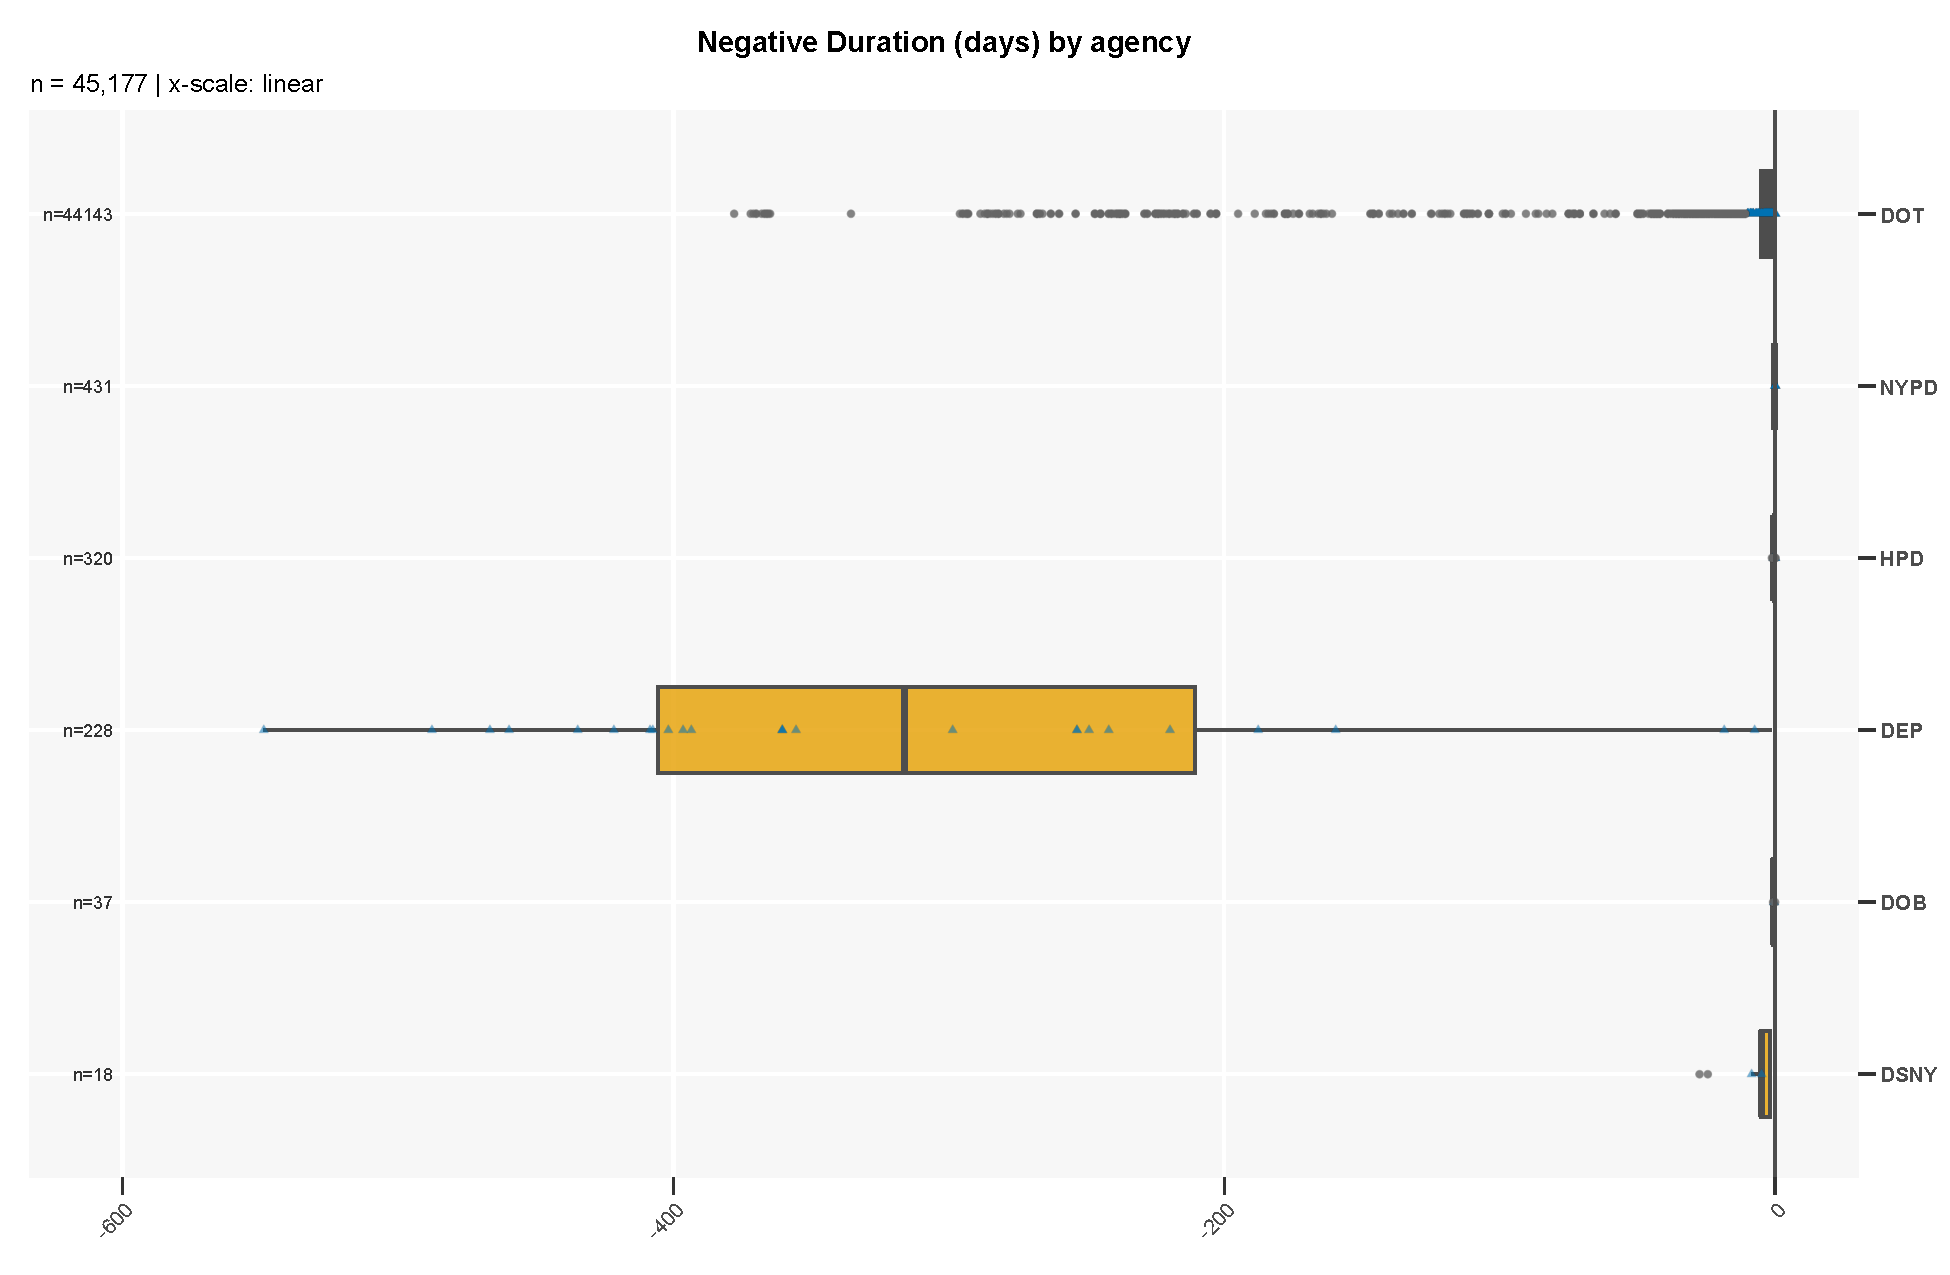
\includegraphics[width=\textwidth, height=0.33\textheight, keepaspectratio]{boxplot_negative_days_by_agency.pdf}
    \caption{311~SRs with negative durations (days) by agency. 
    \textit{Note: pseudo-log scale.}}
    \label{fig:negativedurations}
\end{figure}

Within this group, 115~\textsc{SR}s show extreme negative durations due to 
\texttt{closed\_date} values in the distant past, specifically 
\texttt{1899-12-31} and \texttt{1900-01-01}. 
These records imply durations exceeding $-122$~years. 
Although rare, such outliers can dramatically skew statistical summaries; 
for example, mean calculations become unreliable if not adjusted. 
{\small\emph{(Note: These extreme values likely stem from the well-documented 
SQL default-date anomaly, in which blank or null date fields are coerced to 
the placeholder value \texttt{1900-01-01}. A similar behavior occurs 
in Microsoft~Excel., whose internal date system also begins on January~1,~1900.)}}

Table~\ref{tab:largest-errors} provides a summary of 
\textsc{SR}s with negative durations (in hours). 
Consistent with the broader distribution, the overwhelming majority of 
these cases originate within the Department of Transportation, which 
accounts for approximately \SI{98}{\percent} of all observed errors. 
This concentration reinforces the conclusion that the negative-duration 
anomaly is not evenly distributed across agencies, but rather reflects 
systemic or procedural issues specific to \textsc{DOT}.


\begin{table}[tbp]
    \centering
    \caption{Sample negative durations [excluding extreme values that 
    are lower than $-730$~days]}
    \label{tab:largest-errors}
    \small
    \begin{tabular}{l l r l}
        \toprule
        \texttt{created\_date} & \texttt{closed\_date} & 
        {Duration (hours)} & {Agency} \\
        \midrule
        2024-02-22 13:49:00 & 2023-05-30 13:48:00 & $-6433.02$ & DOT \\
        2020-05-18 15:24:00 & 2020-05-07 15:24:00 & $-264.00$  & DOT \\
        2022-01-10 14:20:00 & 2022-01-06 14:20:00 & $-96.00$   & DOT \\
        2020-05-01 11:33:00 & 2020-04-28 11:33:00 & $-72.00$   & DOT \\
        2021-06-01 11:04:00 & 2021-05-31 10:55:00 & $-24.15$   & DOT \\
        \bottomrule
    \end{tabular}
\end{table}


 \subsubsection{Zero and 1-second Durations:}
\label{subsubsec:zerodurations}
A more prevalent anomaly arises when the \texttt{closed\_date} and 
\texttt{created\_date} share the exact same timestamp to the second. 
This results in a \emph{zero-duration} \textsc{SR}, 
which is inherently nonsensical. 
A total of 387{,}595~zero-duration \textsc{SR}s were identified, 
representing \SI{2.5}{\percent} of all non-blank records. 
Notably, \SI{98}{\percent} of these cases originate from just five agencies—%
the Department of Health~and~Mental~Hygiene (\textsc{DOHMH}), 
Transportation (\textsc{DOT}), Buildings (\textsc{DOB}), 
Environmental~Protection (\textsc{DEP}), and 
Sanitation (\textsc{DSNY}). 
This concentration does not mirror the overall \textsc{SR} distribution 
by agency, suggesting agency-specific data entry or system-level issues.

In addition, another 3{,}460~\textsc{SR}s are recorded as closing within 
one second of their creation. 
While not strictly illogical like negative durations, such 
near-instantaneous closures are highly improbable and represent a 
suspicious pattern, meriting further investigation.

\subsubsection{Suspicious Durations}
\label{subsubsec:suspiciousdurations}
\textbf{Rationale.}  
Service Request (\textsc{SR}) durations are highly right-skewed, 
with some extending months or years. 
Such extremes distort summary measures and hinder comparisons across agencies, 
time periods, or complaint types. 
To ensure interpretable results, a screening procedure was applied 
to identify these \textit{suspicious} durations.

\textbf{Methodology.}  
Durations were truncated to plausible limits: 
2~seconds (excluding zero- and one-second artifacts) to 
172{,}800~seconds (48~hours). 
This reduced the dataset from 15.3~to~10.0~million records 
(\SI{64.9}{\percent} retained) and greatly reduced the long tail. 
Within this subset, five complementary outlier tests were evaluated—
Standard Deviation (SD), Median Absolute Deviation (MAD), 
log-normal thresholds, percentile cutoffs (1–10\%), 
and Interquartile Range (IQR).

\textbf{Findings.}  
Truncation lowered the mean-to-median ratio from~53.7~to~5.2. 
SD, MAD, and IQR tests flagged no further anomalies, 
while log-normal and percentile approaches produced 
operationally reasonable limits. 
The adopted rule—log-normal three–SD cutoff 
($\approx$\,28~seconds)—balanced rigor and interpretability, 
identifying only \SI{0.07}{\percent} of records as outliers. 
This threshold provides a defensible boundary 
between routine and atypical \textsc{SR}s.

\textbf{Summary.}  
A total of 405{,}796~\textsc{SR}s—including 
14{,}741~newly flagged cases—exhibited statistically suspicious or 
operationally implausible durations.

\subsubsection{Positive Durations:}
\label{subsubsec:positivedurations}
While a positive duration is not inherently erroneous, a subset of 
service requests (\textsc{SR}s) exhibit unusually long lifespans. 
five~years (1{,}826~days) were designated as \emph{extreme}.  

A total of 138{,}318~\textsc{SR}s fall into the \emph{large} category (1--2~years). 
These cases are concentrated in three agencies—the Department of 
Parks~and~Recreation (\textsc{DPR}), the Department of 
Health~and~Mental~Hygiene (\textsc{DOHMH}), and the 
Economic~Development~Corporation (\textsc{EDC})—which together account for 
\SI{94}{\percent} of all large-duration \textsc{SR}s. 
The average length of these cases was 1{,}099~days.  

At the more severe end, 1{,}211~\textsc{SR}s qualify as 
\emph{extreme} positive durations ($>$\,5~years). 
Nearly all of these (\SI{94}{\percent}) occurred within \textsc{DPR}. 
The average duration in this group was 1{,}875~days, 
with the maximum recorded at 2{,}009~days.  

\begin{figure}[tbp]
    \centering
    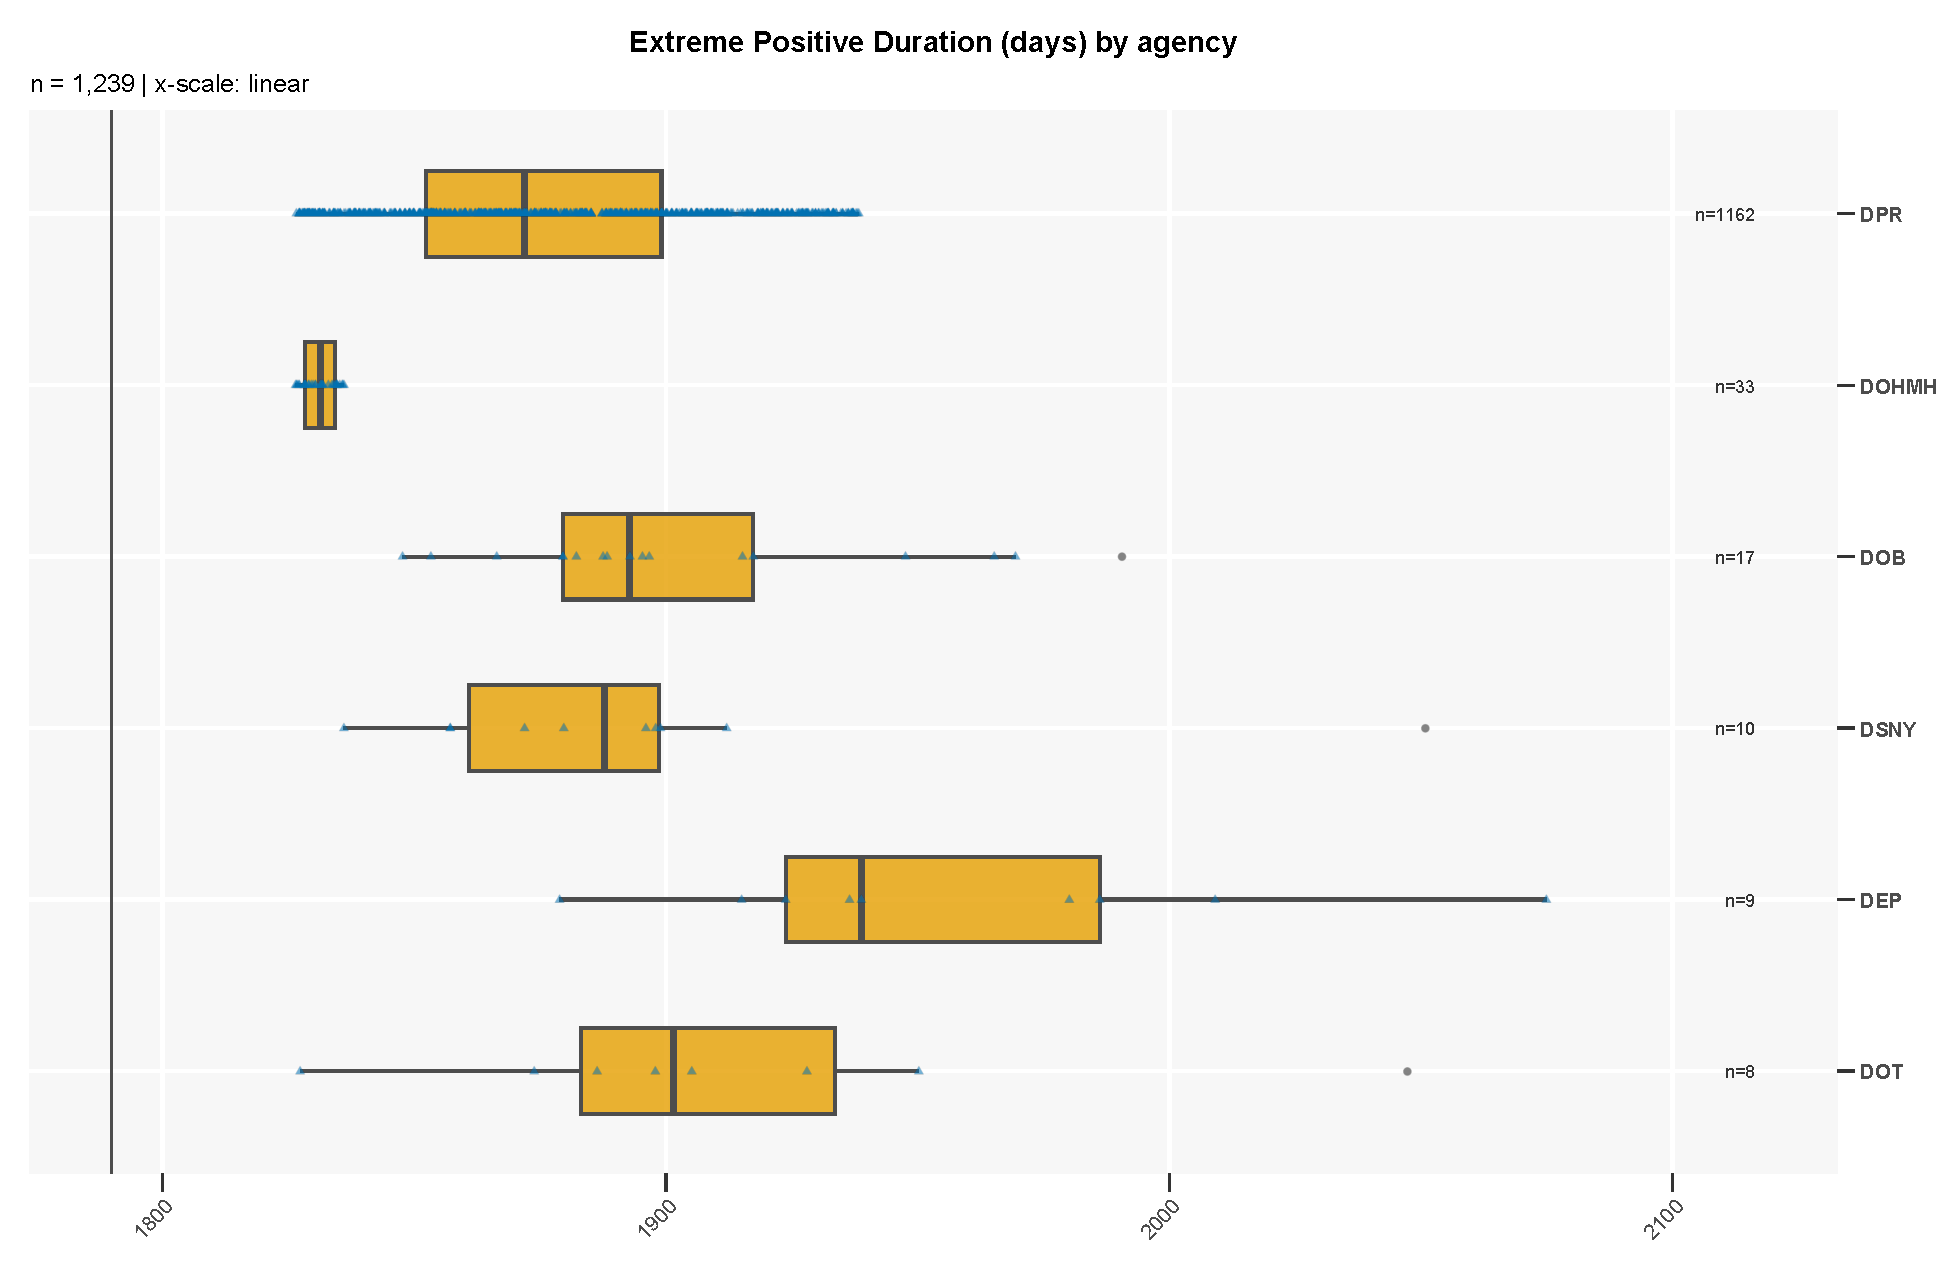
\includegraphics[width=\textwidth, height=0.33\textheight, keepaspectratio]{boxplot_extreme_positive_days_by_agency.pdf}
    \caption{311~service requests (\textsc{SR}s) with extremely large 
    positive durations.}
    \label{fig:extremepositive}
\end{figure}

\subsection{Duplicate \& Redundant Fields}
\label{subsec:redundant}
This analysis revealed several redundant fields, indicating a potential 
need for consolidation and simplification.

\paragraph{\texttt{latitude/longitude} vs.~\texttt{location}}  
The \texttt{location} field is merely a concatenation of the 
\texttt{latitude} and \texttt{longitude} values, enclosed in parentheses 
and separated by a comma. Functionally, it adds no new information yet introduces unnecessary parsing 
complexity. 

While this duplication is relatively benign, it inflates dataset size 
and complicates downstream processing. 
Consolidating these fields—or removing \texttt{location} in favor of the 
atomic \texttt{latitude} and \texttt{longitude} columns—would simplify 
analysis, reduce redundancy, and improve structural coherence.

\paragraph{\texttt{borough} vs.~\texttt{park\_borough}}  
These two fields are entirely redundant, with values matching 
\SI{100}{\percent} across all records. Retaining both 
only increases duplication and introduces potential 
confusion for users.

\paragraph{\texttt{borough} vs.~\texttt{taxi\_company\_borough}}  
Despite their similar names, these fields capture almost entirely distinct 
information, sharing only \SI{0.29}{\percent} of overlapping values. 
The \texttt{taxi\_company\_borough} field appears to be used exclusively 
by the Taxi~and~Limousine~Commission (\textsc{TLC}), suggesting that it 
serves a specialized purpose distinct from the general 
\texttt{borough} designation. This example illustrates 
how field naming conventions can obscure 
specialized agency usage, complicating cross-agency data harmonization.

\paragraph{\texttt{agency} vs.~\texttt{agency\_name}}  
The \texttt{agency} field stores abbreviated identifiers for City agencies 
(e.g.,~\textsc{NYPD}, \textsc{DOT}, \textsc{DSNY}), 
while \texttt{agency\_name} provides their full titles. 
Because the abbreviations are widely recognized and sufficient for most analyses, 
maintaining both fields is, for the most part, redundant. 
Retaining only the abbreviated form would reduce file size and improve efficiency 
without diminishing interpretability.

\paragraph{\texttt{landmark} vs.~\texttt{street\_name}}  
According to the 311~Service~Request (\textsc{SR}) Data Dictionary, 
the \texttt{landmark} field is intended to denote noteworthy sites such as 
parks, hospitals, airports, sports facilities, or performance venues. 
In practice, however, the majority of entries are street names, with 
approximately \SI{60}{\percent} matching the \texttt{street\_name} field. 
Many of the remaining non-matches (excluding blanks) appear to be 
near-equivalents, differing only in spelling or formatting 
(e.g.,~``NINTH~AVE'' vs.~``9~AVE''). 
This pattern suggests frequent misuse of the \texttt{landmark} field and 
underscores its functional redundancy with \texttt{street\_name}. 

\paragraph{\texttt{cross\_street\_1/2} vs.~\texttt{intersection\_street\_1/2}}  
These two street-pair fields are intended to help identify the 
\texttt{incident\_address}. 
Analysis revealed that approximately \SI{84}{\percent} of entries are direct 
duplicates across the two pairs, raising the question of which set should be 
considered authoritative. If the fields are used differently across agencies, 
the lack of documentation leaves their relationship unclear. 
Regardless, the high level of duplication indicates substantial redundancy.  


%-------------------------------------------------------------------------------
%	Sub-section: Reducing File Size
%-------------------------------------------------------------------------------

\subsection{Reducing File Size}
\label{subsec:filesize}
Eliminating duplicate and near-duplicate fields could reduce the 
dataset size by approximately \SI{39.5}{\percent}—a substantial gain. 
The analysis revealed that the following fields could be safely 
removed with minimal loss of information:

\begin{itemize}[left=1.5em]
  \item \texttt{agency\_name}: Redundant with \texttt{agency}, which already uses 
        widely recognized abbreviations.  
  \item \texttt{park\_borough}: Identical to \texttt{borough} and therefore unnecessary.  
  \item \texttt{location}: A concatenation of \texttt{latitude} and \texttt{longitude}, 
        offering no additional analytical value.  
  \item \texttt{cross\_street\_1/2} and \texttt{intersection\_street\_1/2}: 
        With an \SI{84}{\percent} match rate, these fields are highly redundant. 
        Deleting \texttt{intersection\_street\_1/2} is recommended, though this may 
        entail limited information loss.  
\end{itemize}

In addition, certain fields are of limited analytical value because they are sparsely 
populated (\textgreater\SI{99}{\percent} blank). 
These include \texttt{taxi\_company\_borough}, \texttt{road\_ramp}, \texttt{vehicle\_type}, 
\texttt{due\_date}, \texttt{bridge\_highway\_direction}, \texttt{bridge\_highway\_name}, 
\texttt{bridge\_highway\_segment}, and \texttt{taxi\_pick\_up\_location}.  
Although sparse overall, even a \SI{1}{\percent} fill rate corresponds to 
roughly 160{,}000 records in this 16~million-row dataset, suggesting that 
agency-specific analyses may still benefit from these fields. 
A practical approach would be to store such variables in separate, 
agency-level tables.

\paragraph{Field Encoding.}  
Further size reductions can be achieved through categorical encoding. 
For example, rather than storing the text string 
``\texttt{NOISE~--~STREET/SIDEWALK}'' more than 300{,}000~times, 
a numeric or symbolic code could be used instead. 
This approach reduces storage overhead, accelerates processing, and 
improves data quality by eliminating misspellings and other invalid entries. 

\paragraph{Alternative Storage Formats.}  
Beyond structural adjustments, storage efficiency can be substantially improved 
through the adoption of modern columnar data formats. 
Apache~Arrow, a cross-platform, in-memory data framework, enables efficient analytics 
and real-time processing while supporting interoperability across programming languages 
such as~R, Python, and Julia. 
Replacing CSV files with Arrow-based storage can reduce dataset size by orders of magnitude 
while simultaneously improving query performance and computational throughput 
\citep{bates2024csv}.
The integration of columnar storage into open-data publishing pipelines would markedly 
enhance accessibility for analysts while reducing both storage and transmission costs.


%-------------------------------------------------------------------------------
%	Section: Principles
%-------------------------------------------------------------------------------


\section{Principles for Government Open Data Curation}
\label{sec:principles}

Building on the insights gained from the case study of the 
\textsc{NYC 311 SR} dataset, this section articulates a set 
of guiding principles for improving the curation and management of 
government open datasets. 
Derived from the challenges identified in the 311~case study, 
these principles are broadly applicable to other large-scale data 
environments. 
Each principle aims to enhance reliability, efficiency, and usability, 
while promoting transparency and public trust in open-data initiatives. 
Together, they provide a coherent framework for sustainable, 
high-quality open-data governance across both organizational 
and technical boundaries.

\subsection{Principle~1: Establish Cross-Organizational Consistency}
\label{subsec:principle1}

A persistent challenge in government open data is the lack of harmonization 
among agencies in field definitions, formats, and value domains.  
Such inconsistencies distort analyses and impede cross-agency integration.  
To address this, standardized conventions for field naming, categorical 
domains, and formatting must be defined, applied uniformly, and audited 
regularly to ensure continuity as reporting practices evolve.

Equally important is accountability.  
Currently, no entity oversees the quality of NYC’s~311~\textsc{SR} data across 
agencies; each submits independently, allowing anomalies to persist.  
A coordinating governance function—central or distributed—should define, 
monitor, and enforce quality standards.  
Without such oversight, even advanced validation tools risk underuse, 
undermining the credibility and consistency of open data.


\subsection{Principle~2: Ensure Data Entry Accuracy}
\label{subsec:principle2}
Data accuracy and validity are prerequisites for any useful open dataset.  
In the \textsc{NYC~311} case, anomalies such as invalid ZIP codes and 
illogical dates highlight the need for validation at the point of entry.  
Fields should accept only values drawn from authorized domains, with 
software safeguards minimizing human error.  
Key measures include:

\begin{itemize}[left=1.5em]
  \item Auto-generating critical date fields from system events (e.g., status changes);  
  \item Blocking records with implausible sequences, such as a closing date preceding creation;  
  \item Validating structured fields (e.g., agency or ZIP codes) against authoritative references.  
\end{itemize}

Embedding such checks directly in submission workflows reduces systemic 
errors in high-volume datasets and turns quality assurance from a reactive 
activity into a routine operational safeguard.


\subsection{Principle~3: Optimize Storage Efficiency}
\label{subsec:principle3}
Efficient storage and representation are vital for large-scale government 
datasets.  
In the \textsc{NYC~311} case, duplicate or near-duplicate fields inflated 
file size without adding analytic value; removing them could reduce storage 
needs by nearly 40\% while maintaining utility.  

Encoding categorical variables in standardized or numeric formats further 
reduces space, prevents inconsistencies, and simplifies analysis.  
Such optimization lowers storage and transmission costs and improves the 
speed, reliability, and reproducibility of workflows—especially important 
when datasets are widely shared for public use.


\subsection{Principle~4: Maintain and Update Data Dictionaries}
\label{subsec:principle4}
Accurate metadata are vital to the usability of government datasets.  
In the \textsc{NYC~311} case, the Data Dictionary contained undocumented 
fields and outdated domain definitions, creating ambiguity and complicating 
analysis.  

Data Dictionaries should specify data types, valid value domains, and clear 
field definitions, and be reviewed regularly to reflect structural or 
semantic changes.  
Consistent maintenance enables researchers, policymakers, and developers to 
interpret data correctly and supports transparency, reproducibility, and 
trust in open-data resources.


\subsection{Principle~5: Automate Quality Assurance Processes}
\label{subsec:principle5}
Automated validation and quality assurance markedly enhance the reliability 
of government datasets by detecting anomalies in real time.  
In the \textsc{NYC~311} case, spikes in request creation and closure at 
midnight or noon likely reflect batch processes that distort duration 
measures.  Real-time, event-driven validation can prevent such errors at the 
point of entry and surface irregular patterns as they occur.  

Automated routines should flag inconsistencies, illogical sequences, and 
implausible values.  Increasingly, artificial-intelligence (AI) methods—%
including anomaly-detection algorithms for numeric data and natural-language 
models for text fields—complement rule-based checks by identifying subtle or 
rare anomalies that manual review might miss.  
Beyond operational benefits, AI-assisted monitoring strengthens the 
foundation for downstream analytics and machine-learning applications, 
ensuring that training data remain fair, accurate, and actionable.


\subsection{Principle~6: Ensure Data Transparency}
\label{subsec:principle6}
Transparency is a core tenet of open data, requiring that datasets be 
not only accurate but also accessible and comprehensible to a wide 
range of users. This entails publishing clear and complete metadata 
that describe dataset structure, limitations, and intended uses.  
Equally important is open communication about data-quality issues—%
for example, notifying users when systemic anomalies (such as erroneous 
\texttt{closed\_date} values) are identified and explaining how such 
issues will be addressed.  

Proactive transparency fosters trust, promotes accountability, and 
encourages broader civic and research use of datasets.  
By making quality-related information public, agencies transform open 
data from a static disclosure into a participatory process, one in 
which users, analysts, and policymakers collectively contribute to 
continuous improvement and shared understanding.

\subsection{Principle~7: Foster Interoperability and Scalable Access}
\label{subsec:principle7}
Government open data should be distributed in formats that balance public 
accessibility with computational efficiency.  
While flat \texttt{CSV} files remain the universal standard, they become 
inefficient as datasets scale to tens of millions of rows.  

To improve scalability, agencies should offer complementary access options—%
such as structured APIs and columnar formats like Apache Parquet or Arrow—%
while retaining \texttt{CSV} for compatibility.  
Because most agencies already manage data in enterprise systems capable of 
exporting multiple formats, leveraging these infrastructures can serve both 
casual users and high-volume analysts without duplicating effort or risking 
inconsistency.  

Interoperability across formats and platforms ensures that open data remain 
accessible, efficient, and sustainable for long-term public use.


\subsection{Principle~8: Embed Ethical and Privacy Safeguards}
\label{subsec:principle8}

Open-data publication must balance transparency with the protection of 
individual and community privacy.  
Even without direct identifiers, modern data-linkage techniques can 
re-identify individuals by combining open data with other public sources—%
a risk demonstrated in recent studies and government cases.  

To reduce such risks, agencies should apply disclosure-avoidance methods 
such as aggregation, suppression, masking, or differential privacy, and 
conduct ethical reviews for releases containing detailed geospatial or 
temporal information linked to sensitive service categories.  

Integrating privacy safeguards into curation workflows keeps open-data 
programs ethically responsible, legally compliant, and publicly trusted.  
Transparency and privacy are not opposing values but complementary 
pillars of responsible data governance.


\subsection{Synthesis, Outlook, and Actionable Steps}
\label{subsec:actions}
Together, these principles outline a framework for sustaining the reliability 
and integrity of government open data across the full lifecycle of stewardship—%
from harmonization and validation at entry to automation, transparency, and 
ethical accountability.  Although grounded in the \textsc{NYC~311 SR} case, the 
lessons apply broadly wherever open data support public accountability and 
civic innovation.

To move from principle to practice, governments should prioritize 
real-time validation, regular updates to data dictionaries, and standardized 
encoding and storage formats.  Automated checks can flag errors such as 
invalid ZIP codes, detect anomalies as they occur, and reduce reliance on 
manual review.  These measures both improve quality and free staff for 
higher-value analytical work.

Cross-agency and external collaboration is equally vital.  Shared standards, 
metadata, and feedback channels allow issues to be identified and resolved 
transparently while aligning datasets with user needs.  Quality-assurance 
dashboards can continuously monitor key indicators (e.g., missing coordinates 
or invalid codes) and trigger corrective action, reinforcing accountability 
and trust.

Partnerships with data scientists, statisticians, and civic technologists can 
further enhance scalability and methodological rigor, ensuring that validation 
processes remain adaptive and future-proof.  Public-facing initiatives such as 
\textsc{NYC~Open~Data~Week} complement these efforts by promoting data 
literacy, fostering civic engagement, and maintaining feedback loops between 
agencies and the communities they serve.

By embedding these technical and participatory mechanisms, governments can 
transform open-data programs from static repositories into dynamic, trusted 
infrastructures that evolve in quality, transparency, and public value.


%-------------------------------------------------------------------------------
%	Section: Conclusion
%-------------------------------------------------------------------------------

\section{Conclusion}
\label{sec:conclusion}
This study highlights the essential role of systematic anomaly detection and 
robust curation in ensuring the reliability of government open data, using 
New York City’s \textsc{311 SR} dataset as a case study. 
The analysis revealed diverse anomalies—erroneous or missing dates, redundant 
fields, and implausible durations—that, though often subtle, can distort 
results and erode confidence in downstream analyses.

From these findings, we outlined practical principles for improving open-data 
quality: cross-agency consistency, rigorous validation, efficient storage, 
updated documentation, automated quality checks, and transparency. 
Together, these measures provide a roadmap for maintaining the integrity and 
utility of large public datasets.

Although centered on \textsc{NYC 311}, the implications extend to other 
domains such as health, transportation, and environmental monitoring, where 
data inconsistency and incompleteness persist. 
Sound curation is particularly critical for machine-learning applications, 
where biased inputs can compromise accuracy and fairness 
\citep{rahm2000data,geiger2020garbage}. 
The COVID-19 pandemic further underscored the societal need for accurate, 
timely, and trustworthy data 
\citep{worby2020face,khemasuwan2021applications}.

Looking forward, automated validation pipelines and feedback mechanisms will 
be key to sustaining quality at scale. 
Embedding these processes into technical and organizational workflows will 
help transform administrative records into reliable public assets that 
support transparent governance, sound research, and civic innovation.

Ultimately, well-curated data underpin both analytical rigor and public 
trust—without them, the promise of open data cannot be fully realized.


%-------------------------------------------------------------------------------
%	Section: Supplementary Material
%-------------------------------------------------------------------------------

\section*{Supplementary Material}
Extensive supplementary analyses and charts are provided to support 
and extend the findings presented in this paper.  
The full \textsc{R} source code used for dataset prepraration and anomaly detection, 
along with instructions on how to duplicate this analysis—is available at 
\url{https://github.com/jun-yan/nyc311clean}.  
Readers are encouraged to explore this repository for reproducible examples 
and implementation details that complement the discussion in the main text.  

Reference data files, including the 2022--2023 NYC~311~Service Request 
records and supporting USPS ZIP code tables, are available at 
\url{https://doi.org/10.6084/m9.figshare.c.7617311}.  
Together, these materials provide a comprehensive foundation for replicating, 
validating, and extending the analyses described in this study.

\bibliographystyle{jds}
\bibliography{refs}

\end{document}